\documentclass[12pt,a4paper]{article}

% --- STANDARD PACKAGES ---
\usepackage[utf8]{inputenc} % Handle UTF-8 encoding
\usepackage[T1]{fontenc}    % Use modern font encodings
% Set sensible margins (your 4cm was very large)
\usepackage[a4paper, margin=2.5cm]{geometry}

% --- MATH & SYMBOLS ---
\usepackage{amsmath}
\usepackage{amsfonts}
\usepackage{amssymb}

% --- GRAPHICS, TABLES, AND LINKS ---
\usepackage{graphicx} % For images (like your logo and results)
\usepackage{booktabs} % For professional tables (in Results)
\usepackage{hyperref} % For clickable links (GitHub, citations)
\hypersetup{
    colorlinks=true,
    linkcolor=blue,     % color of internal links (e.g., toc)
    citecolor=green,    % color of links to bibliography
    urlcolor=cyan,      % color of external links
    pdftitle={Vulnerability Information System Final Report},
    pdfauthor={Chak Yui Wan, Yicheng Li},
    bookmarks=true      % show bookmarks in PDF viewer
}
% --- REFERENCING (using biblatex) ---
% This is a modern and flexible package for references
% style=authoryear is like Harvard. You could also use style=ieee
\usepackage[style=authoryear, backend=biber]{biblatex}
% Tell biblatex where to find your references
\addbibresource{references.bib}

% --- UTILITY PACKAGES ---
\usepackage{fancyhdr} % For custom headers/footers
\usepackage{lastpage} % For 'Page X of Y'
\usepackage{lipsum}   % For placeholder text (REMOVE THIS LATER)
\usepackage{enumitem} % For custom lists

% --- PAGE STYLE ---
\pagestyle{fancy}
\fancyhf{} % Clear all header and footer fields
\fancyfoot[C]{\thepage\ of \pageref{LastPage}} % Footer: "Page X of Y"
\renewcommand{\headrulewidth}{0pt} % No header line
\renewcommand{\footrulewidth}{0.4pt} % Footer line


%==============================================================================
% --- DOCUMENT START ---
%==============================================================================
\begin{document}

%==============================================================================
% --- TITLE PAGE & ABSTRACT ---
%==============================================================================
    \begin{titlepage}
        \centering
        % --- University Logo ---
        
\includegraphics[width=0.3\textwidth]{UoA_logo_col_vert.jpg}
        \vfill % Add vertical space
        % --- Title ---
        {\Huge \bfseries Vulnerability Information System \\ Final Report}
        \vfill % Add vertical space
        % --- Author/Supervisor Details ---
        {\Large
        \begin{tabular}{r l}
            \textbf{Authors:} & Chak Yui Wan (Student ID: A1870877) \\
            & Yicheng Li (Student ID: A1917736) \\
            \addlinespace[10pt] % Add a 10pt space
            \textbf{Supervisor:} & Hussain Ahmad \\
            \addlinespace[10pt]
            \textbf{Date:} & \today
        \end{tabular}
        }
        \vfill % Add vertical space
        % --- Course Information ---
        {\large
        Report submitted for \\
        \textbf{COMP SCI 3021 – Industry Project in Information Technology}
        }

        \vfill % Add space, pushing abstract towards the bottom

        % --- ABSTRACT (on the Title Page as requested) ---
        \par
        \begin{minipage}{0.9\textwidth} % Constrain width for readability
            \normalsize % Ensure normal font size
            \centering
            {\bfseries Abstract}
            \par\medskip % Add a little space after the heading

            % Must be 150-200 words.
            % Answer: 1. What problem? 2. What approach? 3. What results?
            \noindent % No indentation for the first line
            \lipsum[1] % --- REPLACE THIS with your 150-200 word abstract ---

        \end{minipage}
        \vfill % Fill remaining space
    \end{titlepage}

%==============================================================================
% --- TABLE OF CONTENTS ---
%==============================================================================
    \clearpage
    \pagenumbering{roman} % Use Roman numerals for ToC, List of Figures, etc.
    \tableofcontents
    \clearpage
    \pagenumbering{arabic} % Switch to Arabic numerals for main content
%==============================================================================
% --- 1. INTRODUCTION ---
%==============================================================================
    \section{Introduction}
    % \lipsum[2]
    % You can cite sources like this \parencite{example_book} or this \cite{example_article}.
    \subsection{Background / Context}
    The effective management of cybersecurity risks is a critical priority for modern organisations. Central to this effort is the Common Vulnerabilities and Exposures (CVE) system, which provides a standardised identifier for publicly known security vulnerabilities. Datasets such as the National Vulnerability Database (NVD) aggregate CVE entries with supplementary information, including severity scores (CVSS), affected software, and mitigation links. Timely access to and comprehension of this data are essential for IT professionals and security teams to conduct risk assessments and prioritise remediation efforts. However, the official presentation of this data is typically dense, highly technical, and optimised for in-depth analysis rather than rapid assessment by a broader range of stakeholders.
    \subsection{Motivation}
    This project was motivated by the need for a more accessible and intuitive interface for querying and visualising CVE information. For business clients or IT professionals who are not full-time security analysts, parsing the extensive technical data on standard databases can be time-consuming and cognitively demanding. A significant gap exists for a streamlined tool that can rapidly retrieve, parse, and present the most critical CVE details—such as severity, impact, and affected systems—in a clear, concise, and visually engaging format. This project addresses the demand for a "quick look" solution, enabling users to perform rapid initial assessments without being overwhelmed by technical minutiae.
    \subsection{Proposed Solution}
    To address these challenges, the proposed solution is a full-stack web application built on a three-tier architecture. The presentation layer (front-end) is a static web interface developed with HTML, CSS, and client-side JavaScript, designed to present complex vulnerability data in an intuitive, newspaper-style layout. The application layer (backend) is a custom API developed using Node.js and Express.js. This API serves two primary functions: (1) It queries a local MySQL database to retrieve structured CVE data based on user searches; and (2) It provides an AI-augmented chat service by securely interfacing with the Anthropic Claude 3.5 Sonnet large language model (LLM), passing the relevant CVE data as context for analysis. The data layer consists of a local MySQL database containing a curated CVE_2024 table, which stores the pre-processed vulnerability information for rapid retrieval.
    \clearpage
    \subsection{Key Contributions}
    The primary contributions of this project are:
    \begin{itemize}[label=$\bullet$, leftmargin=*]
        \item Designed and implemented a custom Node.js backend API and a relational MySQL database schema to efficiently store, query, and retrieve specific CVE data.
        \item Developed a highly visual and intuitive front-end interface that transforms complex CVE data into accessible visualisations, including interactive timelines, CVSS score gauges, and risk metric charts.
        \item Integrated a generative AI-powered chat assistant (Anthropic Claude 3.5 Sonnet) that leverages Retrieval-Augmented Generation (RAG) to provide users with contextual, natural-language explanations and analysis of the selected vulnerability.
    \end{itemize}

%==============================================================================
% --- 2. METHODOLOGY / APPROACH ---
%==============================================================================
    \clearpage
    \section{Methodology / Approach}
    The project was executed following a structured, five-phase agile methodology, moving from initial concept to a deployment-ready application. This approach ensured that client requirements were accurately translated into functional software through iterative stages of design, development, and validation.
    \begin{figure}[h!]
        \centering
        % --- 記得換做你張 flowchart 圖 ---
         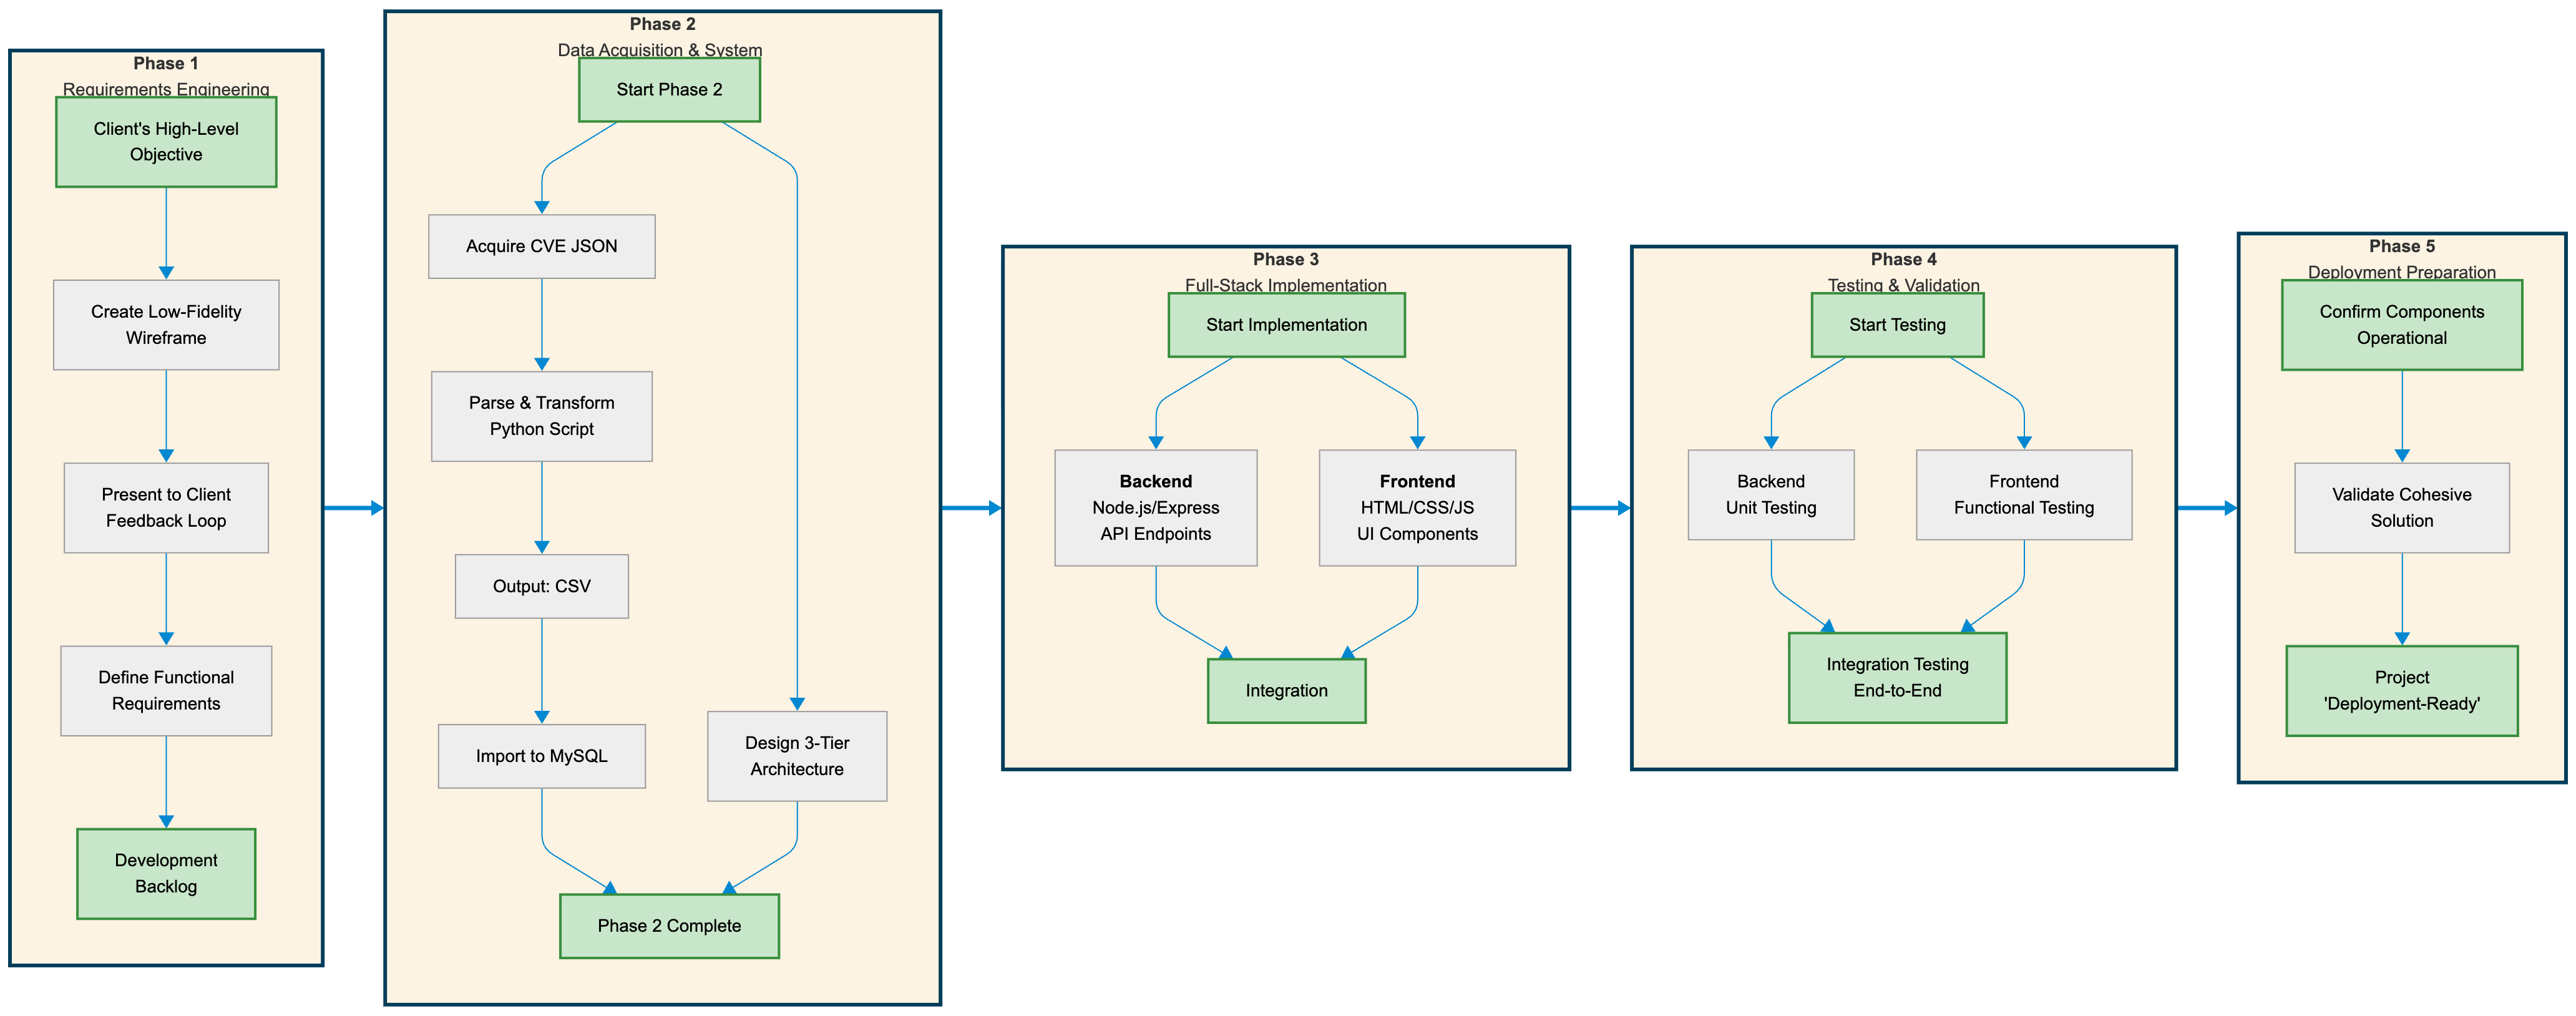
\includegraphics[width=0.8\textwidth]{flowchart-summarising}
%        \fbox{\rule{0pt}{10em}\rule{0.8\textwidth}{0pt}}
        \caption{A flowchart summarizing the project methodology.} % 圖片標題
        \label{fig:methodology} % 俾你喺內文用 \ref{fig:methodology} 嚟 refer 呢張图
    \end{figure}
    \subsection{Requirements Engineering and Prototyping}
    The initial phase involved translating the client's high-level objective—a streamlined CVE search website—into a tangible concept. A low-fidelity, hand-drawn wireframe was created to establish a shared visual understanding of the proposed layout and user journey. This prototype was presented to the client, facilitating a feedback loop that resulted in a concrete set of functional requirements. These requirements were formally defined and categorized into five key visualisation features (e.g., 'CVE Detail Panel', 'Severity Highlight') and six core interaction functions (e.g., 'Complete Search Functionality', 'Search History Cache'), which subsequently served as the development backlog.
    \subsection{Data Acquisition and System Design}
    This phase focused on establishing the data persistence layer and the overall system architecture. The complete 2024 CVE dataset was first acquired in its raw JSON format from the official cve.org repository. Due to the complexity of the nested JSON structure, a custom Python script was developed to parse the data, extract the essential fields (e.g., ID, description, scores, vendors), and transform it into a flattened CSV format. This structured CSV file was then imported into a local MySQL database, which defined the schema for the \texttt{CVE\_2024} table. Concurrently, the 3-tier application architecture was designed, separating the front-end (browser), the backend API (Node.js), and the data layer (MySQL).
    \subsection{Full-Stack Implementation}
    With the architecture and data schema in place, implementation was divided between the two team members to enable parallel development:
    \begin{itemize}[label=$\bullet$, leftmargin=*]
        \item \textbf{Backend Development (Ian):} This workstream focused on building the Node.js/Express server. It involved creating the database connection, writing the SQL queries, and defining the API endpoints (e.g., \texttt{/api/cve/:cveId} and \texttt{/api/cve-chat}) required to serve data to the client application.
        \item \textbf{Frontend Development (Yicheng):} This workstream focused on translating the prototype into a functional user interface. This involved writing the HTML structure, styling with CSS, and developing the client-side JavaScript (\texttt{Enquiry-Search.js}) to handle user input, make asynchronous API calls, and dynamically render the response data into the defined visual components.
    \end{itemize}
    \subsection{Testing and Validation}
    A multi-stage testing strategy was employed to ensure application correctness and stability.
    \begin{itemize}[label=$\bullet$, leftmargin=*]
        \item \textbf{Backend Unit Testing:} The API endpoints were tested directly by accessing their local URLs (e.g., \texttt{http://localhost:3000/api/cve/1001}) to verify correct JSON responses, proper error handling for invalid inputs, and successful database connectivity.

        \item \textbf{Frontend Functional Testing:} The user interface was manually tested to confirm that all specified interaction requirements (e.g., 'Enter Key to Search', 'Loading Spinner') functioned as expected.

        \item \textbf{Integration Testing:} End-to-end tests were performed to ensure the front-end JavaScript correctly fetched data from the backend API and that the data was accurately displayed in the visual components.
    \end{itemize}
    \subsection{Deployment Preparation}
    In the final phase, the application was prepared for demonstration. While not deployed to a public cloud-hosted service, the project was confirmed to be fully 'deployment-ready'. All components (front-end, backend API, and database) were fully configured and operational within a local development environment, validating that the entire stack functions as a cohesive solution.
%==============================================================================
% --- 3. EXPERIMENTAL EVALUATION (if applicable) ---
%==============================================================================
    \clearpage
    \section{Experimental Evaluation}
    This section details the testing environment used to validate the application and presents the final results, analysing how the implemented solution successfully meets the project's objectives.
    \subsection{Experimental Setup}
    The application was tested in a comprehensive, multi-platform local environment to ensure robustness and cross-browser compatibility. The testing setup was configured as follows:
    \begin{itemize}[label=$\bullet$, leftmargin=*]
        \item \textbf{Operating Systems:} macOS 26 Tahoe and Windows 11.
        \item \textbf{Web Browsers:} Google Chrome (\texttt{v128}), Mozilla Firefox (\texttt{v129}), Microsoft Edge (\texttt{v128}), and Apple Safari (\texttt{v18}).
        \item \textbf{Backend Environment:} Node.js \texttt{v24.2.0}.
        \item \textbf{Database Server:} MySQL (\texttt{v8.0}).
    \end{itemize}
    This setup allowed for the validation of the front-end rendering, API connectivity, and backend logic across all major user platforms.
    \subsection{Results and Analysis}
    The project successfully translated the initial low-fidelity concept into a fully functional and visually rich web application.
    \subsubsection{Analysis of Core Visualisation (Prototype vs. Final)}
    Figure \ref{fig:prototype} shows the initial, hand-drawn prototype that served as the foundational blueprint for the user interface. It established the core layout, including a main search, a timeline, a CVSS score gauge, and various metric panels.
    \begin{figure}[h!]
        \centering
        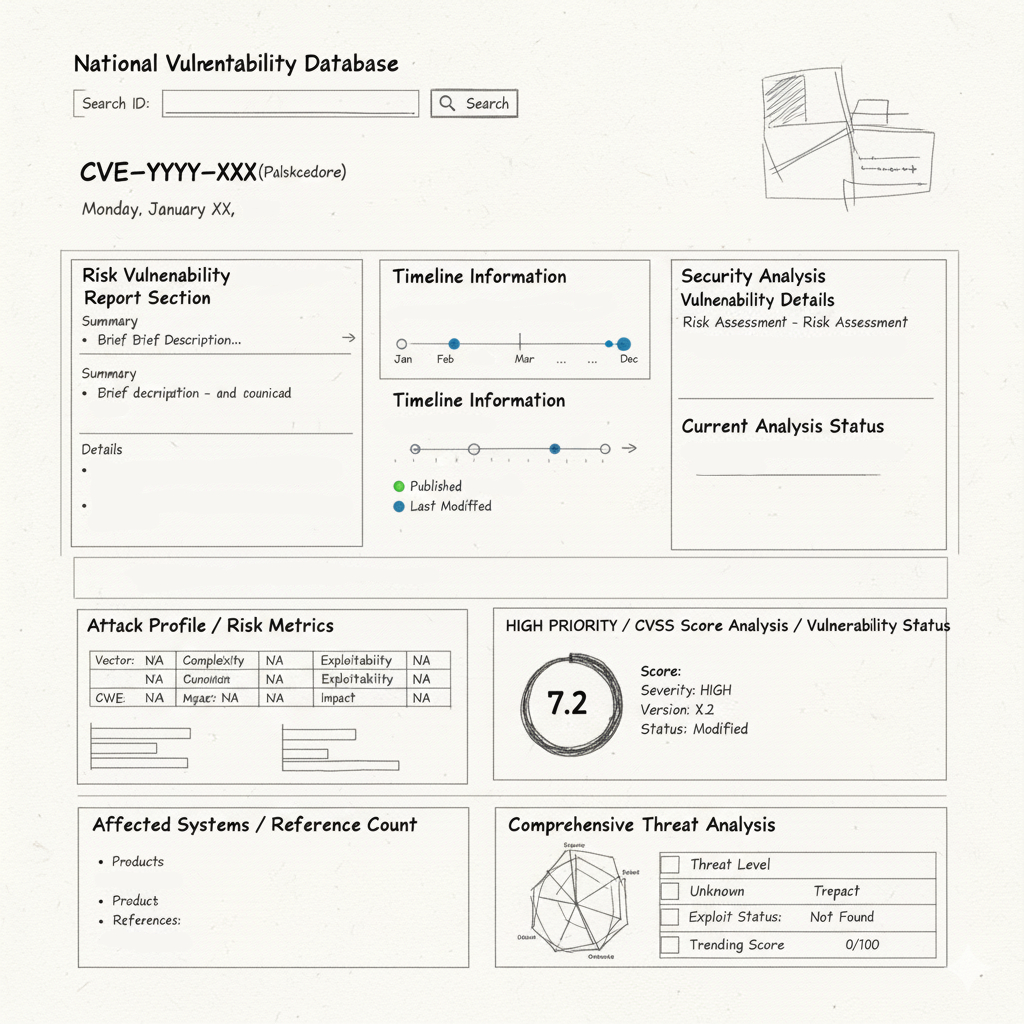
\includegraphics[width=\textwidth]{prototype-website.jpg}
        \caption{Initial Low-Fidelity Prototype}
        \label{fig:prototype}
    \end{figure}
    Figure \ref{fig:final_ui} presents the final implemented user interface, demonstrating a high-fidelity realisation of the initial concept. The final design effectively translates the prototype's wireframes into polished components:
    \begin{figure}[h!]
        \centering
        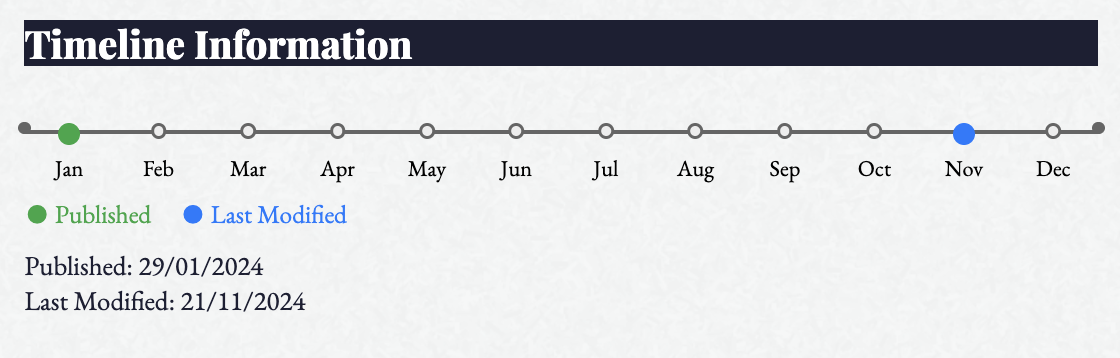
\includegraphics[width=\textwidth]{Timeline-UI}
        \caption{Detailed Implementation of the 12-Month Vulnerability Timeline}
        \label{fig:12_Month_Vulnerability_Timeline}
    \end{figure}
    \begin{figure}[h!]
        \centering
        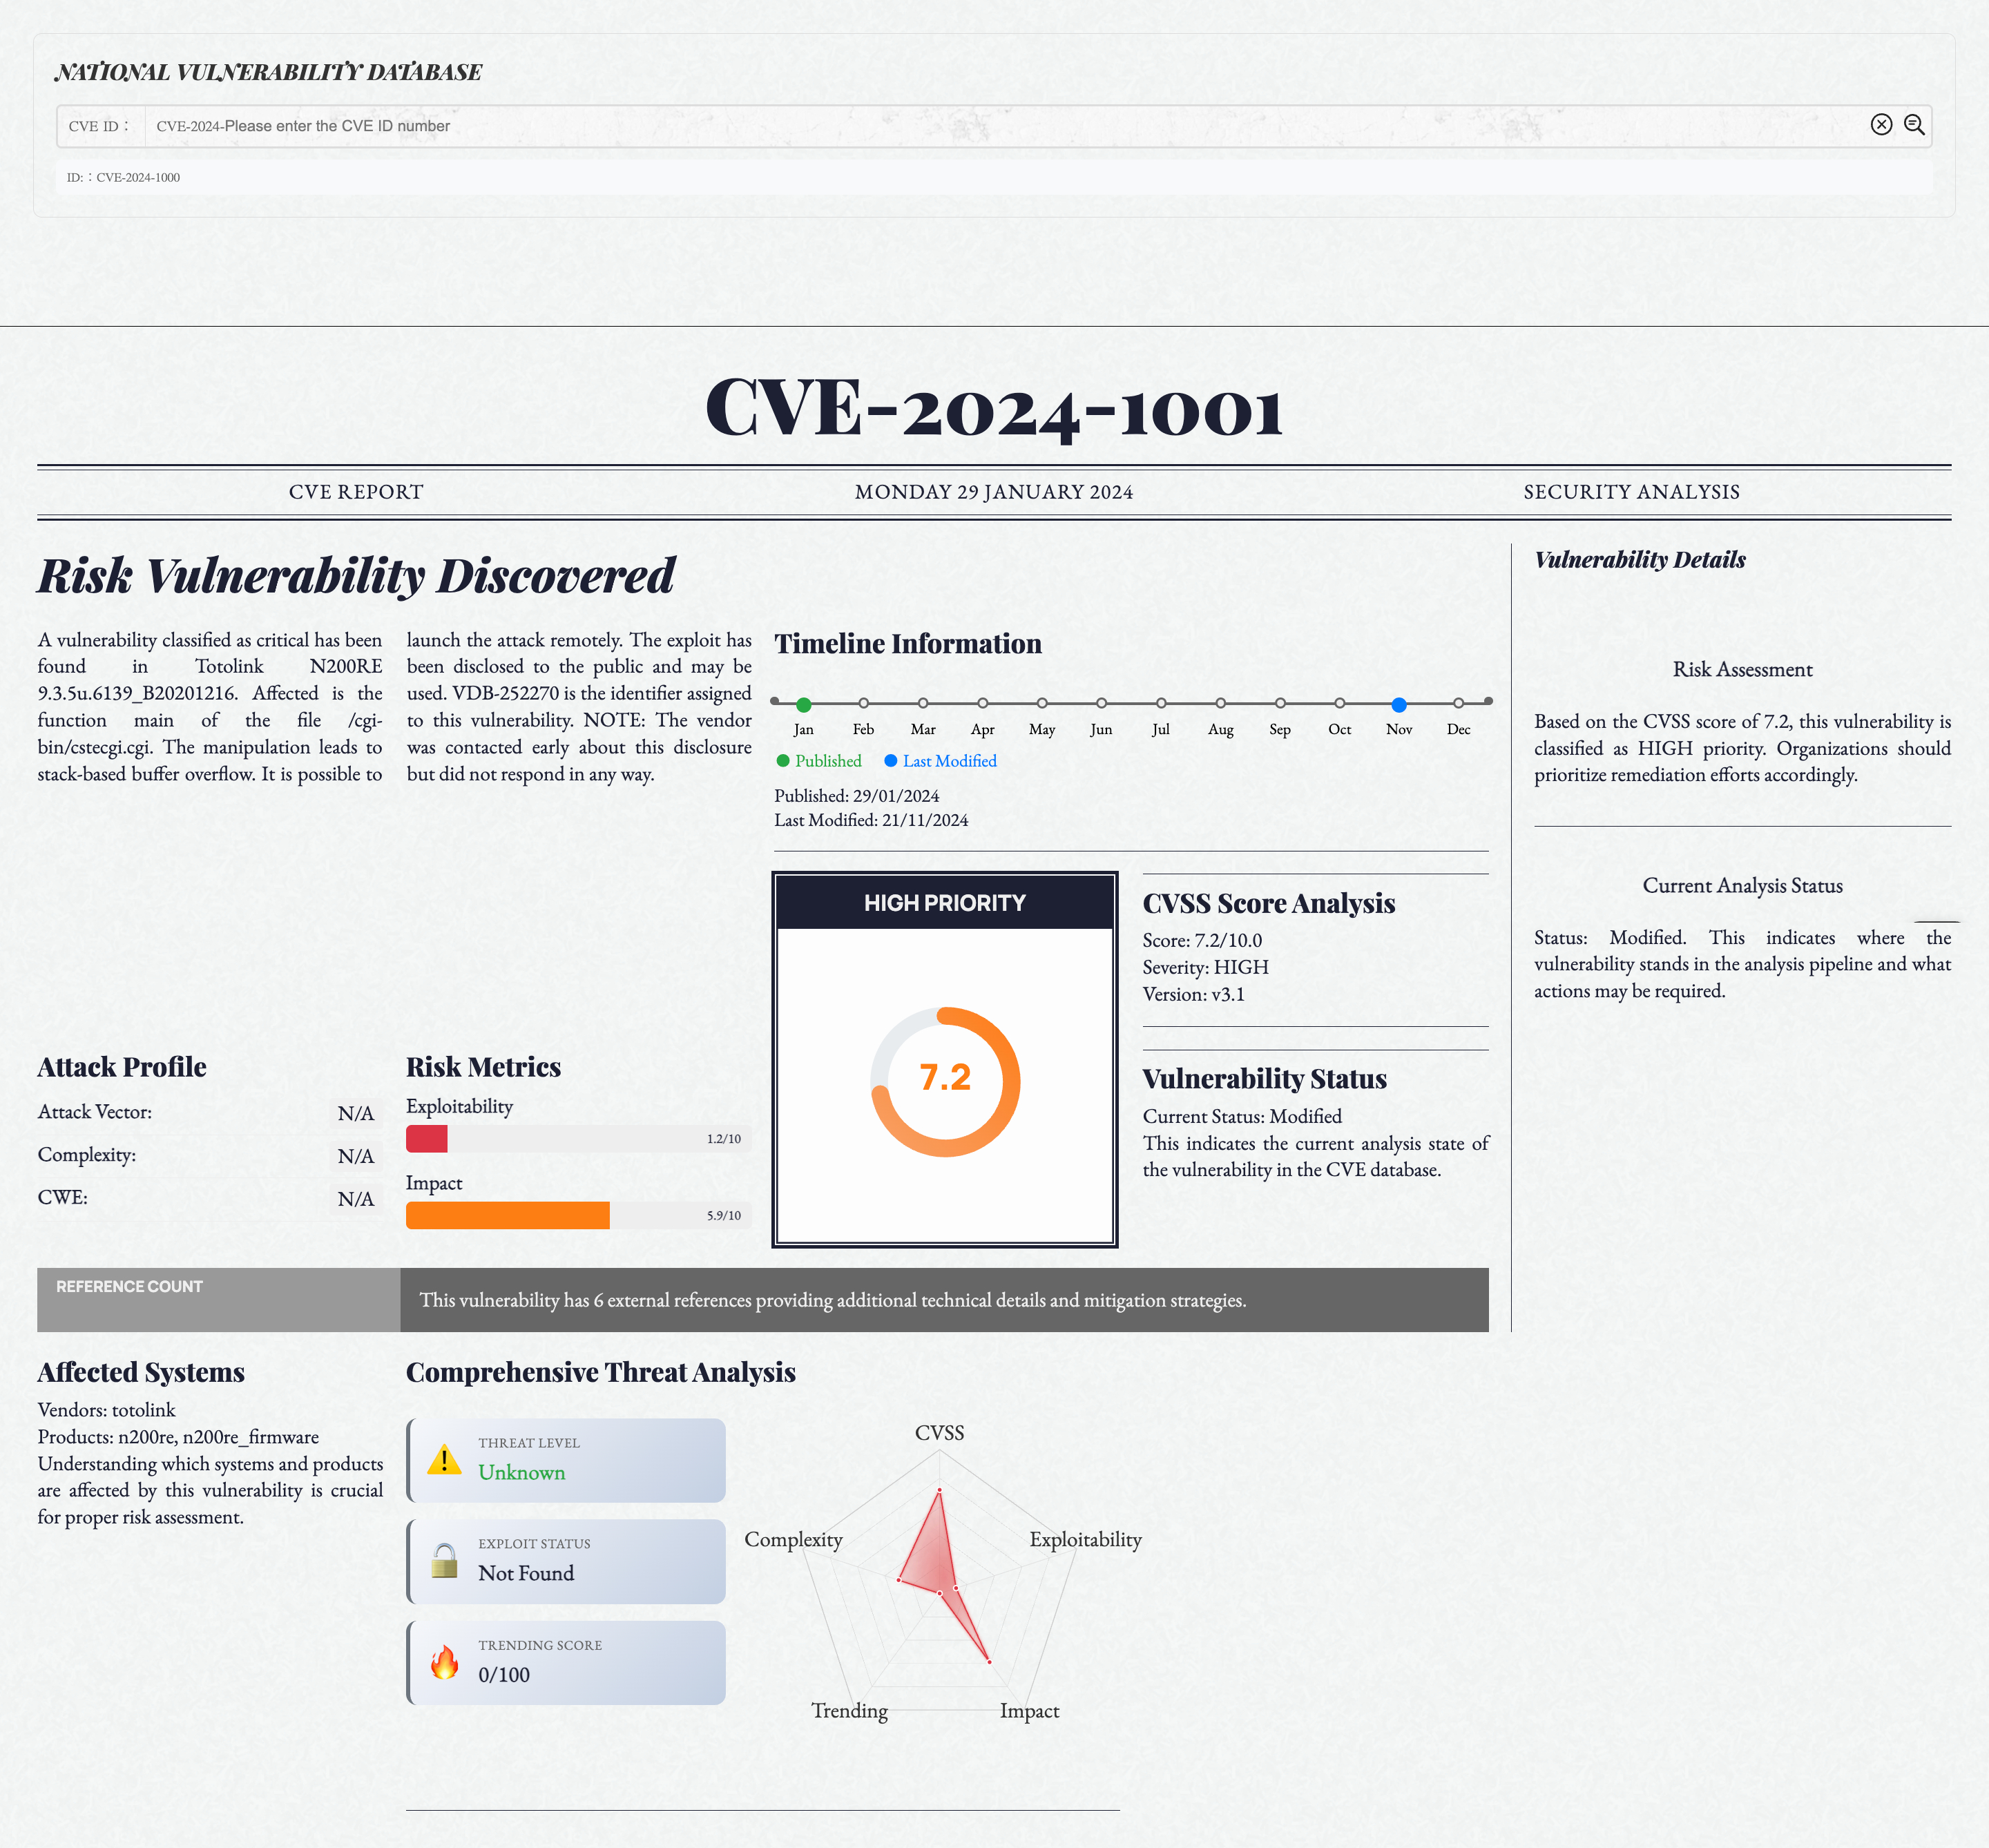
\includegraphics[width=\textwidth]{CVE-Enquiry.jpg}
        \caption{Final Implemented Results Interface}
        \label{fig:final_ui}
    \end{figure}
    \begin{itemize}[label=$\bullet$, leftmargin=*]
        \item \textbf{CVSS Score Analysis:} The simple gauge from the prototype was developed into a dynamic, colour-coded SVG gauge (displaying 7.2 in the example) that immediately communicates the 'HIGH PRIORITY' status.
        \item \textbf{Timeline Information:} The conceptual monthly timeline was implemented as a clean, twelve-month visualisation, clearly marking the 'Published' (Jan 2024) and 'Last Modified' (Nov 2024) dates.
        \item \textbf{Risk Metrics:} The 'Attack Profile' and 'Risk Metrics' tables were implemented as distinct components with clear labels (e.g., Exploitability, Impact) and horizontal bar charts, providing a quick-look assessment of risk factors.
        \item \textbf{Comprehensive Threat Analysis:} The conceptual radar chart was successfully implemented, providing a multi-dimensional view of the threat by plotting metrics for CVSS, Exploitability, Impact, and Trending.
    \end{itemize}
    This direct comparison validates that the core visualisation requirements were met, transforming raw data into an accessible, newspaper-style report.
    \subsubsection{Analysis of Advanced Interaction (AI Assistant)}
    Beyond the static display of data, the project incorporated an advanced interaction feature: a generative AI assistant. As shown in Figure \ref{fig:ai_chatbox}, the 'CVE AI Assistant' is context-aware, loading with information specific to the CVE being viewed (e.g., \texttt{CVE-2024-1001}). It prompts the user with relevant questions, such as "How severe is this vulnerability?" and "What systems are affected?". This feature provides significant added value, allowing users to move beyond simple data consumption and engage in a natural-language dialogue to analyse the vulnerability's implications.
    \begin{figure}[h!]
        \centering
        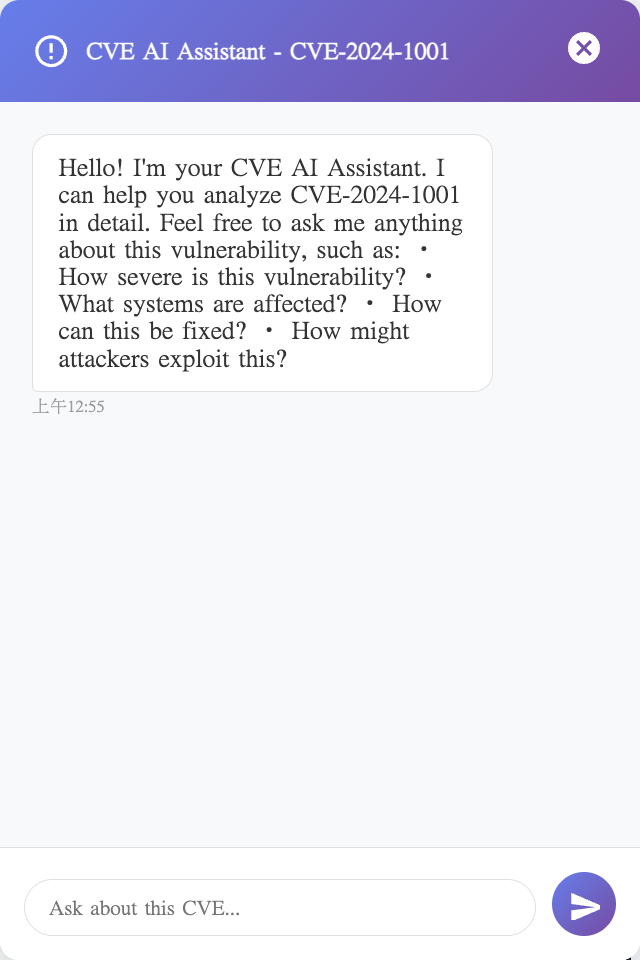
\includegraphics[width=0.8\textwidth]{AI-ChatBox.png}
        \caption{Context-Aware AI Chat Assistant}
        \label{fig:ai_chatbox}
    \end{figure}
%==============================================================================
% --- 4. DISCUSSION ---
%==============================================================================
    \clearpage
    \section{Discussion}
    This section reflects on the project's outcomes, key challenges faced during development, and the practical implications of the solution.
    \\
    \subsection{Project Outcomes and Successes}
    The project was highly successful in achieving its primary goal: transforming dense, technical CVE data into an accessible, user-friendly format. The most effective aspect of the project was the final UI/UX design. By simulating a "newspaper style" layout, the application provides a familiar and intuitive reading experience. This design choice directly addresses the client's "quick look" requirement, as users can rapidly scan headings, gauges, and charts to assess a vulnerability's severity, similar to how one would read a newspaper. The integration of multiple visualisation types—such as the 12-month timeline, CVSS gauge, and risk radar chart—proved to be an effective strategy for converting abstract text values into easily understandable information.
    \\
    \subsection{Challenges Encountered}
    Several challenges emerged during the development process, primarily related to data processing and design decisions:
    \begin{itemize}
        \item \textbf{Data Ambiguity and Processing:} The raw CVE data, acquired as a bulk JSON download, was unexpectedly complex. A significant challenge was parsing this data, as a single CVE entry often contained multiple data objects representing different CVSS versions (v2, v3, v4). Deciding which version to prioritise and developing the Python script to effectively parse and flatten this nested, and at times redundant, data into a clean database schema was a major hurdle. Ultimately, CVSS v3 was selected as the standard for display.
        \item \textbf{Visualisation Design:} A core development challenge was determining the most effective method to visualise abstract data. The team was committed to a highly visual approach, but this required careful consideration of which chart types (e.g., bar, radar, gauge) best represented specific metrics. For example, designing the timeline as a literal 12-month calendar view was a deliberate choice to enhance clarity, but it required more design and implementation effort than a simple text-based date list.
    \end{itemize}
    \subsection{Practical Implications}
    The practical utility of this project is clear. It serves as an effective "first-response" tool for IT professionals, managers, and other stakeholders who need to understand a vulnerability's risk without performing a deep technical dive. By providing a consolidated, high-level dashboard, it accelerates the triage and risk assessment process. Furthermore, the integration of the Claude-powered AI assistant demonstrates a viable path toward Retrieval-Augmented Generation (RAG) in security tools, allowing even non-experts to ask complex questions and receive immediate, context-aware analysis.
%==============================================================================
% --- 5. LIMITATIONS ---
%==============================================================================
    \clearpage
    \section{Limitations}
    % (List and explain at least three limitations)
    \begin{itemize}[label=$\bullet$, leftmargin=*]
        \item \textbf{Technical Constraint:} (e.g., We were limited by...) \lipsum[13]
        \item \textbf{Time Limitation:} (e.g., Due to the project timeline, we could not...) \lipsum[14]
        \item \textbf{Scope Limitation:} (e.g., The project scope did not include...) \lipsum[15]
    \end{itemize}


%==============================================================================
% --- 6. CONCLUSION ---
%==============================================================================
    \clearpage
    \section{Conclusion}
    % Summarise:
    % - What you set out to do
    % - What you achieved
    % - What could be done next (future improvements)
%    \parencite{example_book}
    \cite{example_website}
    \lipsum[16-17]


%==============================================================================
% --- 7. REPLICATION PACKAGE ---
%==============================================================================
    \section{Replication Package}
    The complete source code, documentation, and setup instructions for this project are available at the following publicly accessible GitHub repository:
    \url{https://github.com/ianian-c-y/COMP-SCI-3021---Industry-Project-in-Information-Technology}
    The repository includes a \texttt{README.md} file with detailed instructions for setting up the environment and running the system.

%==============================================================================
% --- REFERENCES ---
%==============================================================================
    \clearpage % Start references on a new page
    % This command prints the bibliography
    \printbibliography[title={References}]

\end{document}